

\documentclass{article}
\usepackage{qilin}
\tikzstyle{process} = [rectangle, rounded corners, minimum width=1.5cm, minimum height=0.5cm,align=center, draw=black, fill=gray!30, auto]
\title{\vspace{-2cm}MAT357: Real Analysis \\ Problem Set 8}
\author{QiLin Xue}
\date{2022-2023}
\usepackage{mathrsfs}
\usetikzlibrary{arrows}
\usepackage{stmaryrd}
\usepackage{accents}
\newcommand{\ubar}[1]{\underaccent{\bar}{#1}}
\usepackage{pgfplots}

\begin{document}

\maketitle
I discussed some problems with Nathan Henry and Jonah Chen.
\begin{enumerate}
    \item Since $A$ and $B$ are compact, we know that $A\cup B$ and $A\cap B$ are also compact. The closure of a compact set is the set itself so by Exercise 12, we can replace $J^*$ with $m.$
    
    Because $A$ and $B$ are measurable, we can write:
    \begin{align}
        m(A) &= m(A \cap B) + m(A \cap B^c) \\ 
        m(B) &= m(B \cap A) + m(B \cap A^c)
    \end{align}
    We now claim that 
    \begin{equation}
        A\cup B = (A\cap B)\sqcup (A\cap B^c) \sqcup (B\cap A^c).
    \end{equation}
    First, we verify that the union is in fact a disjoint union. If an element is in both $A$ and $B$ then it cannot be in any of the complements. If it is in $A\cap B^c$ it is in the complement of $B$ and thus cannot be in the other two sets (which require it to be in $B$). The same goes for $B\cap A^c.$
    
    Next we verify set equality. Note that $A\cup B \subseteq (A\cap B)\sqcup (A\cap B^c) \sqcup (B\cap A^c)$ is true since if an element is in $A$ or $B$, it is either:
    \begin{itemize}
        \item In $A$ and in $B$
        \item Exclusively in $A$
        \item Exclusively in $B$
    \end{itemize}
    Therefore,
    \begin{align}
        m(A) + m(B) &= m(A \cap B) + m(A \cap B^c) + m(B \cap A) + m(B \cap A^c) \\ 
        &= m(A\cap B) + m(A \cap B^c + B\cap A + B\cap A^c) \\ 
        &= m(A\cap B) + m(A\cup B)
    \end{align}
    where in the second line, we used countable additivity.\newpage
    \item \begin{enumerate}[label=(\alph*)]
        \item Let the interval be $I=[a,b].$ It is a basic topological fact that
        \begin{equation}
            \overline{I\setminus A} = I \setminus \text{int}(A) = I \cap (\text{int}(A))^c.
        \end{equation}
        From measurability, we have 
        \begin{align}
            &m(I) = m(I \cap (\text{int}(A))^c) + m(I \cap \text{int}(A)) \\ 
            \implies & |I| = m(\overline{I\setminus A}) + m(\text{int}(A))
        \end{align}
        where we used the fact that $I\cap \text{int}(A) = \text{int}(A)$ since $\text{int}(A) \subseteq I.$ Then by using Exercise 12, and rearranging, we have 
        \begin{equation}
            m(\text{int}(A)) =  |I| - J^*(I\setminus A)
        \end{equation}
        which is by definition $J_*A.$
        \item ??
        \item Theorem 68 states that a function $f:[a,b]\to [0,M]$ is Riemann integrable if and only if the topological boundary of its undergraph is a zero set, $m(\partial(\mathcal{U}f))=0$ and the Riemann-Lebesgue Theorem states that a function $f:[a,b]\to \mathbb{R}$ is integrable if and only if it is bounded and its set of discontinuity points is a zero set.
        
        $\implies:$ Assume that $f:[a,b]\to [0,M]$ is Riemann integrable. Then its topological boundary is a zero set, so we can compute 
        \begin{equation}
            J^*(\mathcal{U}(f)) = m(\overline{\mathcal{U}(f)}) = m(\text{int}(\mathcal{U}(f))) + m(\partial(\mathcal{U}(f))) =  m(\text{int}(\mathcal{U}(f)))  + 0 = J_*(\mathcal{U}(f))
        \end{equation}
        where we used Exercise 12 for the first equality and part (a) for the last equality.

        $\impliedby:$ If the undergraph is Jordan measurable, then $J_*(\mathcal{U}(f)) = m(\text{int}(\mathcal{U}(f)))$ is equal to the outer Jordan measure, i.e. $J^*(\mathcal{U}(f)) = m(\overline{\mathcal{U}(f)}) = m(\text{int}(\mathcal{U}(f))) + m(\partial(\mathcal{U}(f))).$ We have 
        \begin{equation}
            m(\text{int}(\mathcal{U}(f))) = m(\text{int}(\mathcal{U}(f))) + m(\partial(\mathcal{U}(f))) \implies m(\partial(\mathcal{U}(f))) = 0.
        \end{equation}
        By Theorem 68, this means that $f$ is Riemann-integrable.

        Note that Riemann-integrable implies Lebesgue-integrable, and they have the same integral. Therefore, the integral is 
        \begin{equation}
            m(\mathcal{U}(f)) = m(\text{int}(\mathcal{U}(f))) + m(\partial(\mathcal{U}(f))) = m(\text{int}(\mathcal{U}(f))) = J(\mathcal{U}(f))
        \end{equation}
        as desired.
    \end{enumerate}

    \newpage
    \item \begin{enumerate}[label=(\alph*)]
        \item There probably is a very easy way to do so, but I can't see it so here is a full proof.
        
        \textbf{Step 0:} The inner measure of a graph is always zero. See part (e) for a proof.

        \textbf{Step 1:} If $f$ is measurable, and bounded on an open interval $(a,b),$ then the graph of $f$ is measurable. To do so, recall that $f$ is measurable means that the undergraph $\mathcal{U}(f)$ is measurable. We will construct a $G_\delta$ set for $\mathcal{U}(f)$ by defining 
        \begin{equation}
            K_n = \mathcal{U}(f + 1/n)
        \end{equation}
        which clearly satisfies $K_1 \supset K_2 \supset \cdots.$ We claim that 
        \begin{equation}
           \bigcap_{i=1}^{\infty} K_i = \mathcal{U}(f) \bigsqcup G(f) 
        \end{equation}
        where $G(f)$ is the graph of the function. The inclusion 
        \begin{equation}
            \bigcap_{i=1}^{\infty} K_i \supseteq \mathcal{U}(f) \bigsqcup G(f) 
        \end{equation} is true since $\mathcal{U}(f) \subseteq K_i$ and $G(f) \subseteq K_i$ for all $i.$ Now, we need to show that the inclusion holds in the other direction. I wasn't able to entirely figure this part out, but it has to do with the fact that $K_i$ converges to the topological closure of $\mathcal{U}(f)$ and $G(f)$ is a subset of the topological boundary of $\mathcal{U}(f).$
        
        Now that we have set equality, we can use downward measure continuity. We have $K_i \downarrow \mathcal{U}(f) \bigsqcup G(f)$ and $m(\mathcal{U}(f)) < \infty$ (since $f$ is bounded on a bounded interval), so we have
        \begin{equation}
            m(K_i) \downarrow m\left(\mathcal{U}(f) \bigsqcup G(f)\right).
        \end{equation}
        Note that 
        \begin{equation}
            m(K_i) = m(\mathcal{U}(f+1/n)) = m(\mathcal{U}(f)) + (b-a)/n.
        \end{equation}
        Therefore, downward measure continuity givs 
        \begin{align}
            &\lim_{n\to \infty} \left(m(\mathcal{U}(f)) + (b-a)/n \right)= m(\mathcal{U}(f)) + m({G}(f)) \\ 
\implies & m(\mathcal{U}(f)) = m(\mathcal{U}(f)) + m(G(f)) \\ 
\implies & 0 = m(G(f))
        \end{align}
        % We can also write 
        % \begin{align}
        %     \bigcap_{i=1}^{\infty} K_i &= \bigcap_{i=1}^{\infty} \left(\mathcal{U}(f) \bigsqcup (a,b) \times [0,1/n]\right) \\ 
        %     &= \mathcal{U}(f) \bigsqcup \bigcap_{i=1}^{\infty} (a,b) \times [0,1/n].
        % \end{align}
        % Therefore,
        % \begin{align}
        %     m^*\left(\bigcap_{i=1}^{\infty} K_i\right) &= m^*\left(\mathcal{U}(f) \bigsqcup \bigcap_{i=1}^{\infty} (a,b) \times [0,1/n]\right) \\ 
        %     &= m^*(\mathcal{U}(f)) + m^*\left(\bigcap_{i=1}^{\infty} (a,b) \times [0,1/n]\right) \\
        %     &= m^*(\mathcal{U}(f)) + 0,
        % \end{align}
        % where the last line is because the areas of the rectangles decrease to zero, i.e. $\lim_{n\to \infty}(b-a)/n = 0.$ By property (b) of Theorem 1, we have 
        % \begin{align}
        %     & m^*\left(\mathcal{U}(f) \bigsqcup G(f) \right) \le m^*(\mathcal{U}(f)) \\ 
        %     \implies & m^*(\mathcal{U}(f)) + m^*(G(f)) \le m^*(\mathcal{U}(f)) \\
        %     \implies & m^*(G(f)) = 0.
        % \end{align}
        % If the outer and inner measure of the graph are both zero, then the graph is measurable with measure $0.$
        % \textbf{?????}

        \textbf{Step 3:} If $f$ is measurable and bounded on $\mathbb{R}$, then the graph of $f$ is measurable. To prove this, we can partition $\mathbb{R}$ into the intervals $(-n,n)$ for $n\in \mathbb{N}.$ Define $f_n(x):(-n,n)\to \mathbb{R}_{>0}$ to be the function $f$ restricted to $(-n,n).$ Then $f_n$ is measurable since 
        \begin{equation}
            \mathcal{U}(f_n) = \mathcal{U}(f) \cap (-n,n) \times (-\infty,\infty)
        \end{equation}
        Because $\mathcal{U}(f)$ and $(-n,n) \times (-\infty,\infty)$ are both measurable, then $\mathcal{U}(f_n)$ must be measurable. By Step 2, we also have that $G(f_n)$ is measurable. We can write 
        \begin{equation}
            G(f) = \bigcup_{n=1}^{\infty} G(f_n)
        \end{equation}
        and by countable subadditivity, we have 
        \begin{equation}
            m(G(f)) \le \sum_{n=1}^{\infty} m(G(f_n)) = 0,
        \end{equation}
        so the graph of $f$ is measurable.

        \textbf{Step 4:} If $f$ is measurable, then the graph of $f$ is measurable. To do this, consider the map 
        \begin{equation}
            T: (x,y) \mapsto (x, \tanh(x))
        \end{equation}
        which is a diffeomorphism, so it is a meseomorphism. Note that $\tanh$ maps 
        \begin{equation}
            [0,a) \mapsto [0,\tanh a]
        \end{equation}
        and $\tanh^{-1}$ maps
        \begin{equation}
            [0,a) \mapsto [0, \tanh^{-1} a].
        \end{equation}
        Therefore, $T$ maps 
        \begin{equation}
            \mathcal{U}(f) \mapsto \mathcal{U}(\tanh \circ f).
        \end{equation}
        Because $\mathcal{U}(f)$ is measurable, its image is measurable, so the graph $G(\tanh \circ f)$ is measurable by Step 3, since $\tanh \circ f$ is bounded. Similarly, the preimage of $G(\tanh \circ f)$ is $G(f)$, and since $T$ is a meseomorphism, then $G(f)$ must be measurable.

        \item This is false. Recall that there exists a non-measurable set $A \subseteq [0,1].$ Then define 
        \begin{equation}
            f(x) = \chi_{A}(x) = \begin{cases}
                1 & x \in A \\ 
                0 & x \notin A
            \end{cases}
        \end{equation} 
        The graph is a zero set since it is a subset of $\{0,2\} \times \mathbb{R}$ which itself is a zero set. However, the function is measurable since the undergraph 
        \begin{equation}
            \mathcal{U}(f) = A \times [0,1)
        \end{equation}
        is not measurable. This is because if it was measurable, then for all $X$
        \begin{equation}
            m^*X = m*(\mathcal{U}(f) \cap X) + m^*(\mathcal{U}(f) \cap X^c)
        \end{equation}
        But we can let $X$ take on the form of $X = Y \times [0,1),$ where $Y\subseteq [0,1]$ to get 
        \begin{equation}
            m^*X = m^*(Y) = m^*(A \cap Y) + m^*(A \cap Y^c).
        \end{equation}
        But because $A$ is non-measurable, the above is not always true, so $\mathcal{U}(f)$ is not measurable, and therefore $f$ is non-measurable.
        \item Not assigned.
        \item Suppose the measurability hypothesis was not necessary. Then by the zero slice theorem, any graph is measurable since every vertical slice of a graph contains exactly 1 point, so it is a zero slice almost everywhere.
        
        However, by part (c), there exists a graph that is not measurable. It has an inner measure of $0,$ so the outer measure must be positive. Therefore, the graph is not of measure $0$ and the ``modified'' zero slice theorem does not hold.
        \item The inner measure in $\mathbb{R}^2$ is defined using closed rectangles:
        \begin{equation}
            m_*(X) = \text{sup}\left\{\sum_k |R_k| : \{R_k\} \text{ are disjoint and } R_k \in X\right\}.
        \end{equation}
        However, the only possible closed rectangles that are contained in a graph is a point and a horizontal line. Since $\{R_k\}$ is a countable collection of zero sets, then by countable additivity $\sum_k |R_k| = 0$ and so $m_*(G(f))=0.$
        \item Consider the uncountable collection $\{X_\alpha\}$ where $\alpha \in \mathbb{R}_{>0}$ and 
        \begin{equation}
            X_\alpha = G(f) + \alpha
        \end{equation}
        with $f$ being the function defined in part (c), which has a graph with infinite outer measure, so each $X_\alpha$ has infinite outer measure. The $X_\alpha$ are also disjoint since they are all a constant shift from one another.
    \end{enumerate}

    \newpage
    \item \begin{enumerate}
        \item Refer to the following diagram.
        
        \begin{center}
            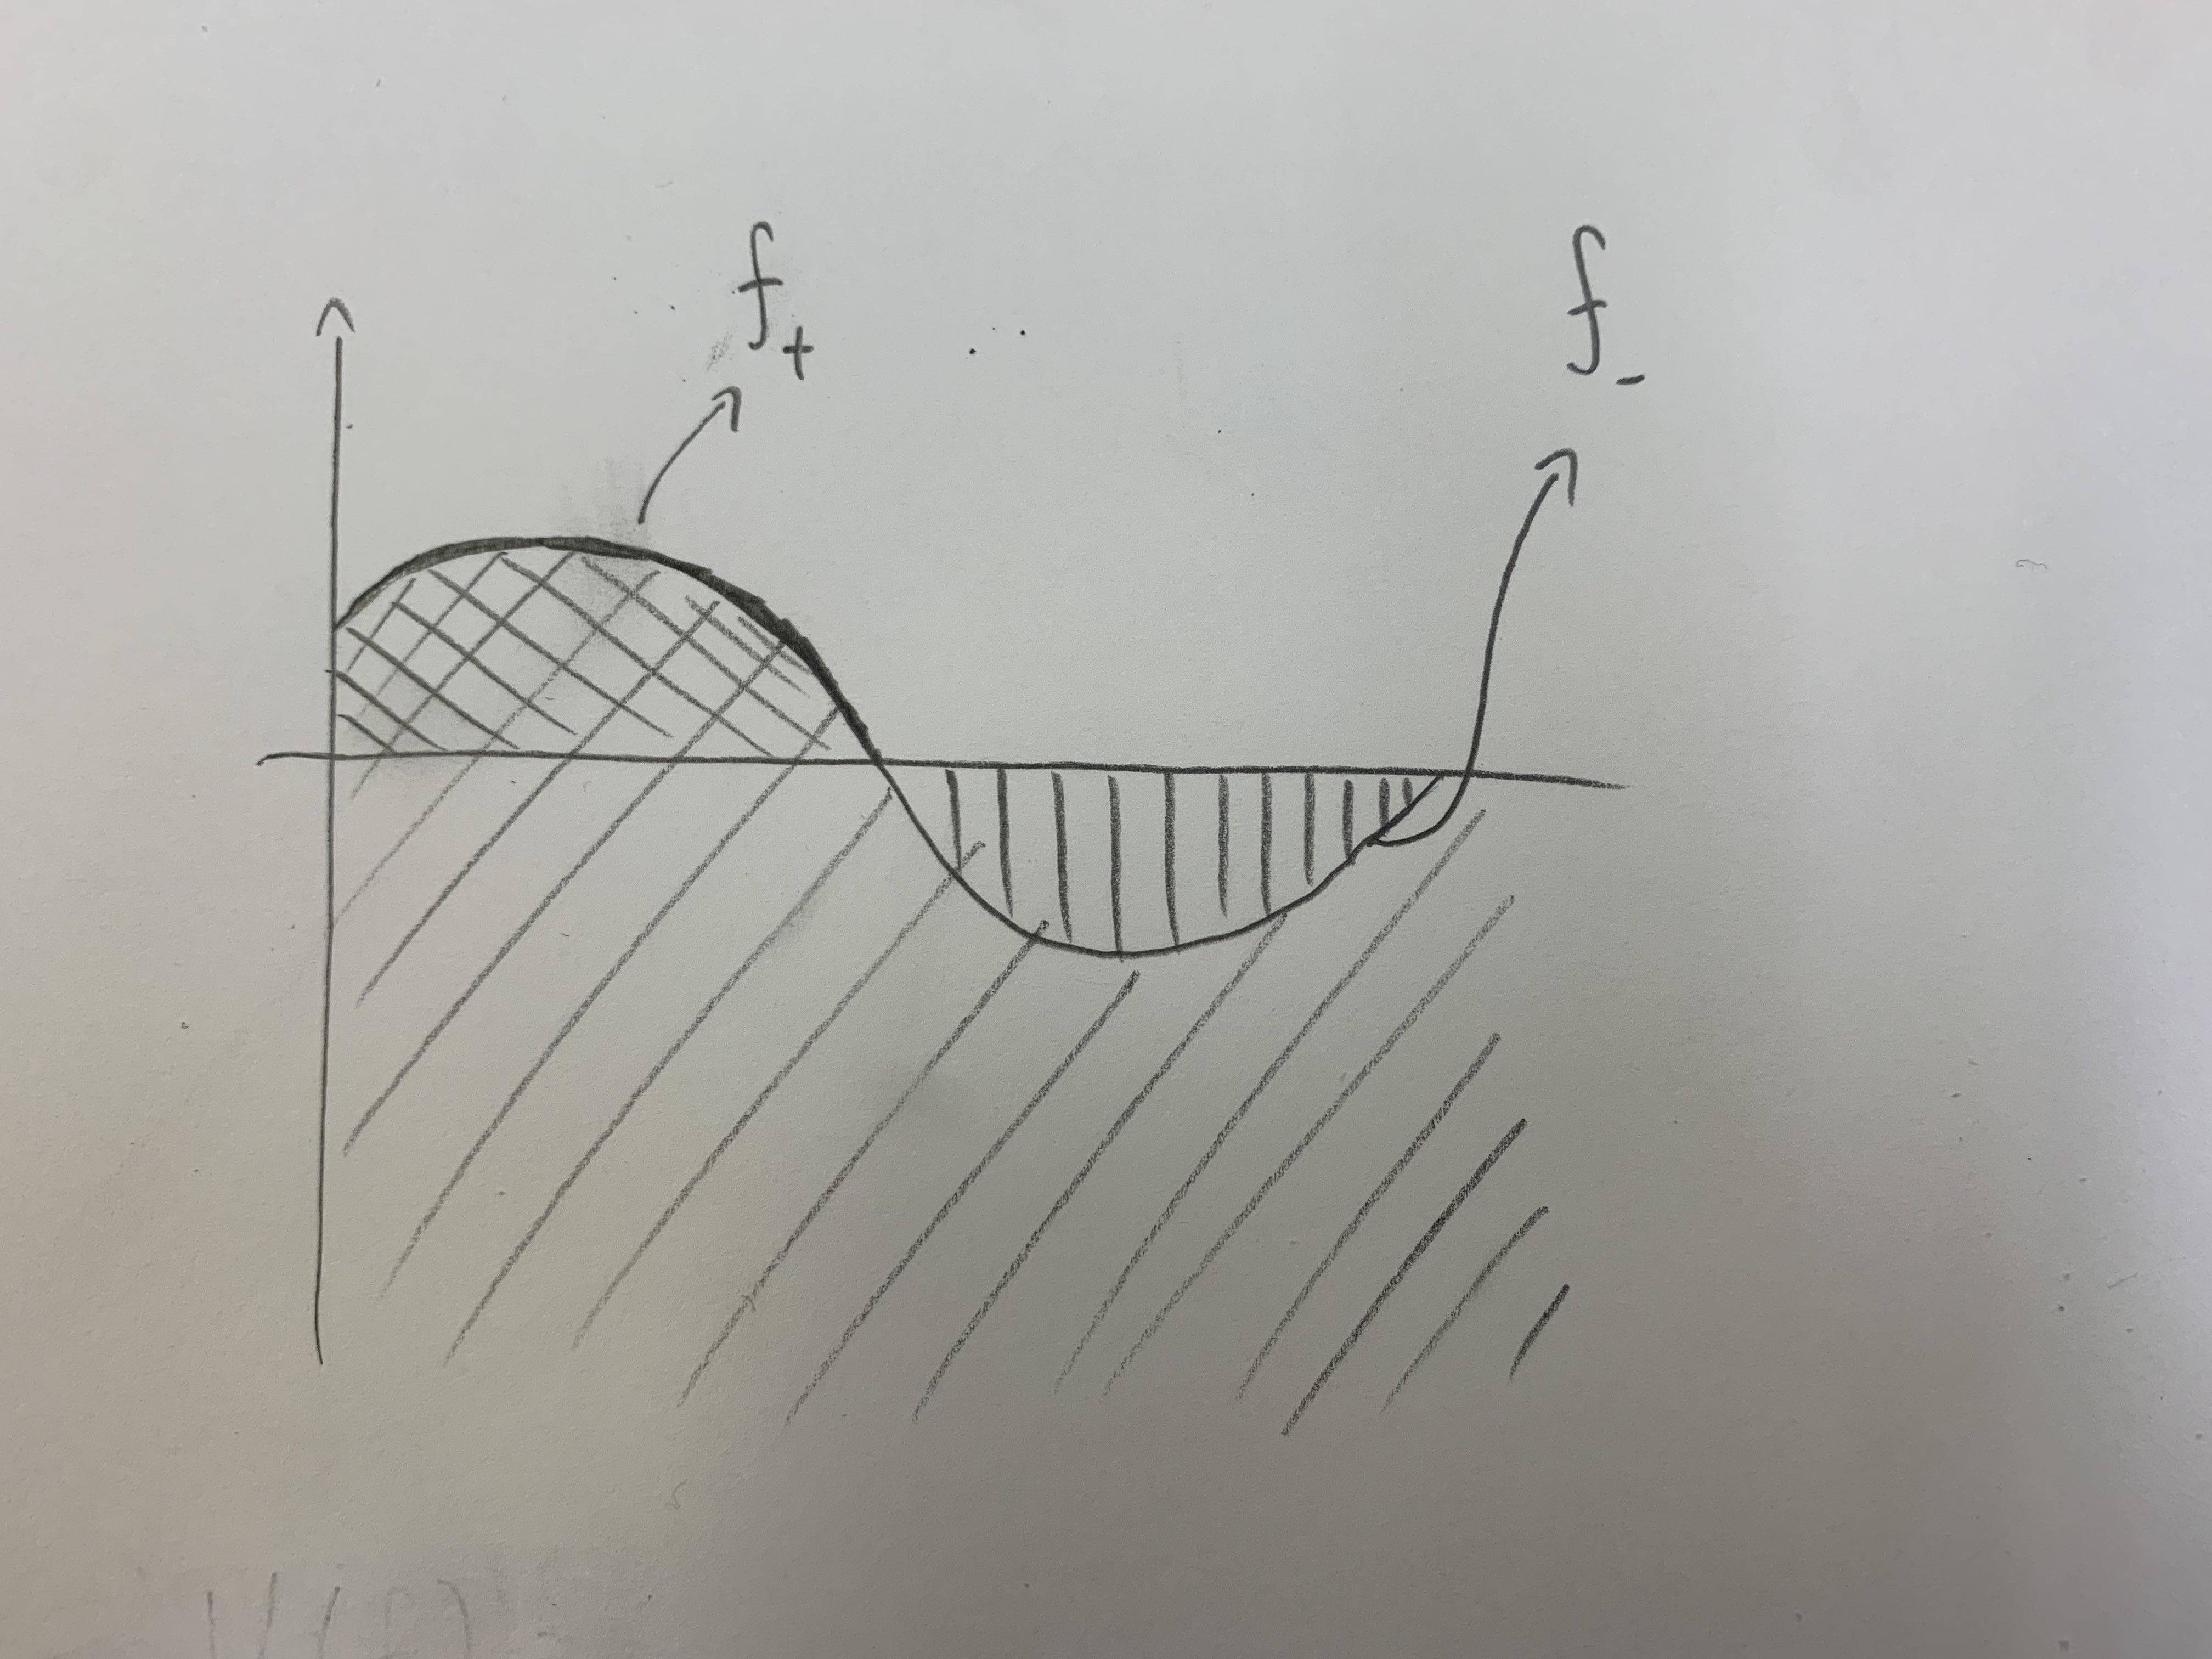
\includegraphics[width=0.8\textwidth]{pset8_graph.jpg}
        \end{center}
        The total undergraph can be written as 
        \begin{equation}
            \underline{\mathcal{U}}(f) = \mathcal{U}(f_+) + H_- + \mathcal{U}(f_-) + G(f_-)
        \end{equation}
        where we are defining the undergraph of a negative function as 
        \begin{equation}
            \mathcal{U}(f_-) = \{(x,y) \in \mathbb{R}^2 : 0 \ge y > f(x)\}
        \end{equation}
        and $H_-$ as the bottom half plane. We first prove that $f_+,f_-$ being measurable implies that $\underline{\mathcal{U}}(f)$ is measurable.

        We proved in class that $H_-$ is measurable. By assumption, $\mathcal{U}(f_+),\mathcal{U}(f_-)$ are measurable, and by question 2, $G(f_-)$ is measurable, and because measurable sets forms a $\sigma$-algebra, then $\underline{\mathcal{U}}(f)$ is measurable.
        
        Next we prove that $\underline{\mathcal{U}}(f)$ is measurable implies that $f_+,f_-$ are measurable. We can write
        \begin{equation}
            {\mathcal{U}}(f_+) = \underline{\mathcal{U}}(f) \cap (H_-)^c
        \end{equation}
        Again, because measurable sets forms a $\sigma$-algebra, then ${\mathcal{U}}(f_+)$ is measurable. Similarly, $f_-$ is measurable since 
        \begin{equation}
            {\mathcal{U}}(f_-) = \underline{\mathcal{U}}(f) \cap (H_+)^c.
        \end{equation}
        \item Consider $T:(x,y) \mapsto (x,1/y).$ The image of $\mathcal{U}(f)$ under this transformation is 
        \begin{equation}
            T(\mathcal{U}(f)) = \mathcal{O}(1/f)
        \end{equation}
        where we are defining $\mathcal{O}(1/f) = \{(x,y): 1/f(x) < y\}$ to be the overgraph.

        Note that this transformation fixes $x$ so to prove this, we can look at a simpler one-dimensional example. The map $x \mapsto 1/x$ is a diffeomorphism, so it maps connected intervals to connected intervals. Specifically, it maps 
        \begin{equation}
            (0,a) \mapsto (1/a,\infty).
        \end{equation}
        For clarity, note that we can also define 
        \begin{equation}
            \mathcal{O}(1/f) = (\underline{\mathcal{U}}(1/f) + G(1/f))^c.
        \end{equation}
        Because $T$ is a diffeomorphism, it is a lipeomorphism, so it is a meseomorphism and sends measurable sets to measurable sets. Since $f$ is measurable, $\mathcal{U}(f)$ is measurable, so $\mathcal{O}(1/f)$ is measurable. We can write
        \begin{equation}
            \underline{\mathcal{U}}(1/f) = \mathcal{O}(1/f)^c \cap G(1/f)^c.
        \end{equation}
        Note that $G(1/f)$ is measurable since the meseomorphism sends $G(f)$ to $G(1/f).$ Therefore, the total undergraph of $1/f$ is measurable and by part (a), we know that $1/f$ is measurable.
        \item We first show that if $f$ is measurable then $\log f$ is measurable. Note that the map $T:(x,y) \mapsto (x,\log y)$ has a continuous derivative and its inverse also has a continuous derivative, so it is a lipeomorphism and is thus a meseomorphism. Note that $\log$ maps
        \begin{equation}
            (0,a) \mapsto (-\infty, \log a)
        \end{equation}
        so $T$ maps 
        \begin{equation}
            T: \mathcal{U}(f) \mapsto \hat{\mathcal{U}}(\log f).
        \end{equation}
        By proposition 28, $\hat{\mathcal{U}}(\log f)$ is measurable if and only if $\mathcal{U}(\log f)$ is measurable, which implies $\log f$ is measurable. Similarly, $\log g$ is also measurable.
        \begin{lemma}
            If $a,b:\mathbb{R} \to (0,\infty)$ is measurable, then $a+b$ is measurable.
            \begin{proof}
                Not only are they measurable, but they have the same measure. This is something we covered in class, as part of the Theorem that 
                \begin{equation}
                    \int a + \int b = \int (a+b)
                \end{equation}
                where we are using the Lebesgue measure, which is defined as 
                \begin{equation}
                    \int a = m(\mathcal{U}(a)).
                \end{equation}
            \end{proof}
        \end{lemma}
        By the above lemma, $\log f+\log g$ is measurable, so $\log fg$ is measurable. Now it remains to show that if $h$ is measurable, then $e^h$ is measurable. To do so, consider the inverse map 
        \begin{equation}
            T^{-1}: (x,y) \mapsto (x,e^y)
        \end{equation}
        which is also a meseomorphism. Note that $e^x$ maps 
        \begin{equation}
            (0,a) \mapsto (1,e^a)
        \end{equation}
        so $T^{-1}$ maps 
        \begin{equation}
            T: \mathcal{U}(h) \mapsto \mathcal{U}(e^h) \cap (\mathbb{R} \times (0,1))^c
        \end{equation}
        The image is measurable and $(\mathbb{R} \times (0,1))$ is measurable, so $\mathcal{U}(e^h)$ is measurable, so $e^h$ is measurable. Therefore, let $h = \log(fg),$ which we've already shown is measurable. Then by the previous part, $e^h = fg$ is measurable, and we're done.
    \end{enumerate}

    \newpage
    \item Note that the standard definition is exactly just part (a). First, we show that (a) and (b) are equivalent. If the preimage of every closed ray is measurable, then we can write 
    \begin{equation}
        f^{-1}((a,\infty)) = f^{-1}\left(\bigcap_{n=1}^{\infty}(a-1/n,\infty)\right) = \bigcap_{n=1}^{\infty} f^{-1}(a-1/n,\infty).
    \end{equation}
    A countable intersection of measurable sets is measurable. Similarly, we can write 
    \begin{equation}
        f^{-1}([a,\infty)) = f^{-1}\left(\bigcup_{n=1}^{\infty}[a+1/n,\infty)\right) = \bigcup_{n=1}^{\infty} f^{-1}[a-1/n,\infty).
    \end{equation}
    A countable union of measurable sets is measurable. Now we will prove the loop of implications:
    \begin{equation}
        (k) \implies (f) \implies (a)\&(b) \implies (i) \implies (k)
    \end{equation}
    \textbf{Proving $(k)\implies (f)$:} every open interval is a $G_\delta$ set since we can write any open set as an infinite union of open sets, $(a,b) = \bigcup_{i=1}^{\infty}(a,b).$

    \textbf{Proving $(f) \implies (a)\&(b)$:} We can write $(a,\infty)=\bigcup_{n=1}^{\infty}(a, a+n).$ Then:
    \begin{equation}
        f^{-1}(a,\infty) = f^{-1}\left(\bigcup_{n=1}^{\infty}(a, a+n)\right) = \bigcup_{n=1}^{\infty} f^{-1}(a, a+n).
    \end{equation}
    A countable union of measurable sets is measurable. We've already shown that (a) and (b) are equivalent, so this shows that (f) implies (a) as well.

    \textbf{Proving $(a)\&(b) \implies (i)$:} Because $\mathbb{R}$ is separable, any open set can be written as a disjoint union of open sets. We can write 
    \begin{equation}
        A = \bigcup_{i=1}^{\infty} (a_i,b_i) = \bigcup_{i=1}^{\infty} (a_i,\infty) \cap [b_i,\infty)^c.
    \end{equation}
    Then:
    \begin{equation}
        f^{-1}(A) = f^{-1}\left(\bigcup_{i=1}^{\infty} (a_i,\infty) \cap [b_i,\infty)^c\right) = \bigcup_{i=1}^{\infty} (f^{-1}(a_i,\infty) \cap f^{-1}[b_i,\infty)^c).
    \end{equation}
    From (a) and (b), $f^{-1}(a_i,\infty)$ and $f^{-1}[b_i,\infty)$ are measurable, so $f^{-1}(a_i,\infty) \cap f^{-1}[b_i,\infty)^c$ is measurable. Therefore, $f^{-1}(A)$ is measurable since a countable union of measurable sets is measurable.

    \textbf{Proving $(i)\implies (k)$:} We can write any $G_\delta$ set $G$ as 
    \begin{equation}
        G = \bigcup_{i=1}^{\infty} A_i
    \end{equation}
    where the $A_i$ are open sets. Then:
    \begin{equation}
        f^{-1}(G) = f^{-1}\left(\bigcup_{i=1}^{\infty} A_i\right) = \bigcup_{i=1}^{\infty} f^{-1}(A_i).
    \end{equation} 
    A countable union of measurable sets is measurable, so $f^{-1}(G)$ is measurable.

    We are now done. Note that in our proof, we used the fact that $f^{-1}$ commutes with countable unions and countable intersections. This is a basic topology fact, so we have used it without proof.
\end{enumerate}
\end{document}